\documentclass[11pt]{article}
\usepackage[margin=1in]{geometry}
\usepackage{amsmath,amssymb,amsthm}
\usepackage{graphicx}
\usepackage[hidelinks]{hyperref}

\newtheorem{theorem}{Theorem}
\newtheorem{lemma}{Lemma}
\newtheorem{remark}{Remark}

\newcommand{\Env}{\operatorname{Env}}
\newcommand{\Stab}{\operatorname{Stab}}
\newcommand{\Fix}{\operatorname{Fix}}
\newcommand{\Isom}{\operatorname{Isom}}
\newcommand{\alg}{\mathrm{alg}}
\newcommand{\borel}{\mathcal B}

\title{A Counterexample to Directed Unions for Algebraic Envelopes}
\author{Run \texttt{fa\_banach\_001}, agent \texttt{agent\_lane\_04}}
\date{June 14, 2026}

\begin{document}
\maketitle

\section*{Status}

\textbf{Claimed counterexample.}  The construction below gives a negative
answer to the question in Ferenczi--Lopez-Abad, \emph{Envelopes in Banach
spaces}, arXiv:2112.11795, asking whether the directed-union formula for
isometric envelopes remains true for algebraic envelopes.

\section*{Source Problem}

The source paper proves the following directed-union formula for the isometric
envelope.

\begin{center}
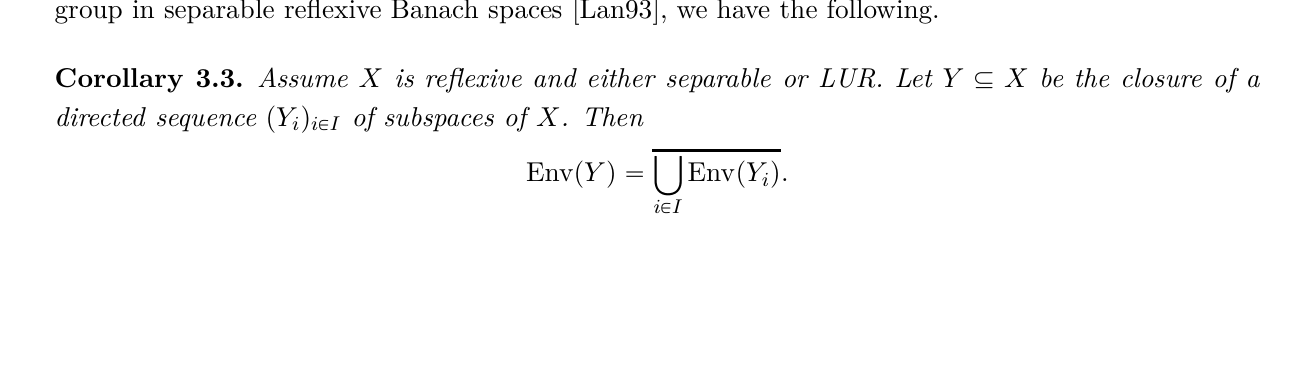
\includegraphics[width=\linewidth]{figures/open_problem_context_p19.png}
\end{center}

Immediately after it, the authors ask whether the analogous statement holds
for algebraic envelopes.

\begin{center}
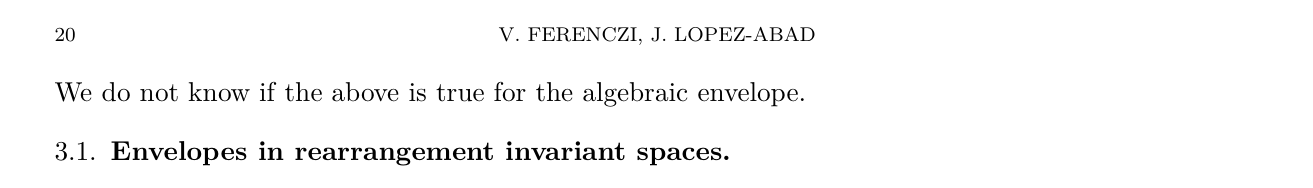
\includegraphics[width=\linewidth]{figures/open_problem_question_p20.png}
\end{center}

In the notation of the source paper, the algebraic envelope of a subspace
\(Y\subseteq X\) is
\[
  \Env^{\alg}(Y)=\Fix(\Stab_{\Isom(X)}(Y)),
\]
the subspace of all vectors fixed by every surjective linear isometry of \(X\)
which fixes \(Y\) pointwise.

Thus the question is whether, when \(X\) is reflexive and separable or LUR and
\(Y=\overline{\bigcup_i Y_i}\) for a directed family of subspaces,
\[
  \Env^{\alg}(Y)
  =
  \overline{\bigcup_i \Env^{\alg}(Y_i)}
\]
must hold.

\section*{Idea of the Proof}

Finite-dimensional sublattices of \(L_p\) have no hidden algebraic envelope:
inside each atom of the finite partition, measure-preserving isometries can
move equal-measure pieces around, so a fixed function must be constant on each
atom.

The limit sublattice below is different.  It remembers the first coordinate of
\([0,1]\times\{0,1\}\), but not the two-point fiber.  Because the two fiber
weights are unequal, any measure automorphism that fixes every base set must
also fix each sheet of the two-point fiber.  Therefore the indicator of one
sheet is fixed by all isometries stabilizing the limit subspace, even though it
is not itself base-measurable.  This creates a strict algebraic envelope at the
limit while all finite-stage envelopes stay trivial.

\section*{Counterexample}

\begin{theorem}
Let \(1<p<\infty\), \(p\ne 2\).  There are a separable reflexive space
\(X\) and an increasing sequence of subspaces \(Y_n\subseteq X\), with
\[
  Y=\overline{\bigcup_{n=1}^\infty Y_n},
\]
such that
\[
  \overline{\bigcup_{n=1}^\infty \Env^{\alg}(Y_n)}=Y
  \quad\text{but}\quad
  \Env^{\alg}(Y)\supsetneq Y.
\]
Consequently the directed-union formula for algebraic envelopes is false.
\end{theorem}

\begin{proof}
Let
\[
  \Omega=[0,1]\times\{0,1\},\qquad
  \mu=\lambda\otimes\left(\frac13\delta_0+\frac23\delta_1\right),
\]
where \(\lambda\) is Lebesgue measure.  Put \(X=L_p(\Omega,\mu)\).  This is a
real separable reflexive \(L_p\)-space.  Since \(\Omega\) is a standard nonatomic
probability space, \(X\) is isometric to the usual \(L_p[0,1]\).

Let \(\mathcal A\) be the base sigma-algebra
\[
  \mathcal A=\{E\times\{0,1\}:E\in\borel([0,1])\},
\]
and let \(Y=L_p(\mathcal A)\).  For \(n\ge 1\), let \(\mathcal A_n\) be the
finite sigma-algebra generated by the dyadic intervals of length \(2^{-n}\) in
the first coordinate, again with the whole two-point fiber attached.  Set
\[
  Y_n=L_p(\mathcal A_n).
\]
Then \(Y_n\) is increasing and \(\overline{\bigcup_nY_n}=Y\).

We first show that \(\Env^{\alg}(Y_n)=Y_n\).  Let \(f\notin Y_n\).  Then on
some atom \(C\) of \(\mathcal A_n\), the restriction of \(f\) is not essentially
constant.  Hence there are real numbers \(a>b\) and positive-measure sets
\(B,C'\subseteq C\) of equal measure such that \(f\ge a\) on \(B\) and
\(f\le b\) on \(C'\).  As \(C\) is nonatomic, there is a measure-preserving
automorphism of \(\Omega\) that swaps \(B\) and \(C'\), is the identity outside
small pieces of the atom \(C\), and preserves every atom of \(\mathcal A_n\).
The induced composition isometry of \(L_p(\Omega)\) fixes \(Y_n\) pointwise but
does not fix \(f\).  Therefore no \(f\notin Y_n\) lies in
\(\Env^{\alg}(Y_n)\), and \(\Env^{\alg}(Y_n)=Y_n\).

It follows that
\[
  \overline{\bigcup_n\Env^{\alg}(Y_n)}
  =
  \overline{\bigcup_nY_n}
  =
  Y.
\]

Now let
\[
  A_0=[0,1]\times\{0\}.
\]
We claim that \(\mathbf 1_{A_0}\in \Env^{\alg}(Y)\).  Let \(T\) be a surjective
linear isometry of \(L_p(\Omega,\mu)\) fixing \(Y\) pointwise.  Since
\(\mathbf 1_\Omega\in Y\), \(T\mathbf 1_\Omega=\mathbf 1_\Omega\).  By the
Banach--Lamperti description of \(L_p\)-isometries for \(p\ne2\), \(T\) is
therefore induced by a measure-algebra automorphism \(\theta\) of \(\Omega\).
Because \(T\) fixes \(Y=L_p(\mathcal A)\) pointwise, \(\theta\) fixes every
base set \(E\times\{0,1\}\).

Let \(B=\theta(A_0)\).  For every Borel \(E\subseteq[0,1]\),
\[
  \mu\bigl(B\cap(E\times\{0,1\})\bigr)
  =
  \mu\bigl(A_0\cap(E\times\{0,1\})\bigr)
  =
  \frac13\lambda(E).
\]
Disintegrate over the first coordinate.  For a.e. \(x\), the fiber
\(B_x\subseteq\{0,1\}\) has conditional measure in
\(\{0,\frac13,\frac23,1\}\).  The preceding identity for all \(E\) says that
this conditional measure is \(\frac13\) a.e.  Hence \(B_x=\{0\}\) for a.e.
\(x\), and so \(B=A_0\) in the measure algebra.  Thus \(T\mathbf 1_{A_0}
=\mathbf 1_{A_0}\).

Since this holds for every surjective isometry fixing \(Y\) pointwise,
\(\mathbf 1_{A_0}\in\Env^{\alg}(Y)\).  But \(\mathbf 1_{A_0}\notin Y\), because
it is not measurable with respect to the base sigma-algebra \(\mathcal A\).
Therefore \(\Env^{\alg}(Y)\supsetneq Y\), as required.
\end{proof}

\section*{Verification Notes}

The proof uses no computation.  The finite-stage step uses only the
nonatomicity of each atom of the finite base partition.  The limit-stage
strictness uses the unequal conditional weights \(1/3\) and \(2/3\), which make
the sheet \(A_0\) recognizable among all measurable subsets after conditioning
on the base.

The Banach--Lamperti theorem is used only in the standard form that a
surjective linear isometry of \(L_p\), \(p\ne2\), is a weighted composition
operator; since the isometry fixes the constant \(1\), the weight is \(1\).

\section*{Novelty Check}

Before promotion, I searched the run indexes for arXiv `2112.11795`, envelope,
algebraic envelope, fixed-point subalgebra, and directed-union terms.  The only
hits were the prior unfinished attempt for this same route and unrelated uses
of the words `envelope' or `centralizer'.

I also searched the web for exact and close phrases including:
\begin{itemize}
\item \texttt{"We do not know if the above is true for the algebraic envelope"},
\item \texttt{"algebraic envelope" "directed" "union" "Banach"},
\item \texttt{"Env\string^alg" "directed" "union"},
\item \texttt{"Env\string^{alg}" "L\_p" "fixed-point subalgebra"}.
\end{itemize}
No later paper or explicit answer to this question was found in that bounded
search.  The counterexample is close to the source paper's own fixed-point
subalgebra obstruction, but the source does not instantiate the unequal-fiber
example above.

\section*{Limitations}

This packet disproves the directed-union formula for algebraic envelopes.  It
does not address whether additional assumptions, such as WOT-closedness of the
relevant stabilizer or a fixed-point hypothesis on the limiting sigma-algebra,
recover a positive theorem.

\section*{Human Review Recommendation}

Review the Banach--Lamperti reduction and the conditional-fiber calculation
showing that a base-fixing measure automorphism must fix \(A_0\).  These are
the only non-formal points in the counterexample.

\begin{thebibliography}{9}

\bibitem{FLA}
V.~Ferenczi and J.~Lopez-Abad,
\emph{Envelopes in Banach spaces},
arXiv:2112.11795.

\bibitem{Lamperti}
J.~Lamperti,
\emph{On the isometries of certain function-spaces},
Pacific J. Math. \textbf{8} (1958), 459--466.

\end{thebibliography}

\end{document}
